\documentclass[10pt,twocolumn]{article}
\usepackage[letterpaper,margin=0.75in,columnsep=0.3in]{geometry}
\usepackage[T1]{fontenc}
\usepackage{newtxtext,newtxmath}
\usepackage{microtype}
\usepackage{graphicx}
\usepackage{booktabs}
\usepackage{xcolor}
\usepackage[numbers,sort&compress]{natbib}
\usepackage[hidelinks]{hyperref}
\usepackage[font=small,labelfont=bf]{caption}
\usepackage{enumitem}
\usepackage{float}
\setlist{nosep,leftmargin=1.2em}
\setlength{\tabcolsep}{4pt}
\newcommand{\sys}[1]{\textit{#1}}

\title{\textbf{Notably, Everything Changed:\\ How the Prose of Computer Science Papers Shifted after ChatGPT and GPT-4}}
% TODO: affiliation and contact before posting.
\author{Chengxu Bian}
\date{October 2026}

\begin{document}
\maketitle

\begin{abstract}
We measure how the writing of published computer science papers changed across 2016--26. We analyze the body text of 9,472 papers from ten venues across systems, machine learning, AI, vision, language and databases (OSDI, NSDI, MLSys, VLDB, NeurIPS, ICML, ICLR, AAAI, CVPR, ACL), plus post-era arXiv versions of COLM and EuroSys papers. From 2024 on, papers more often contain wording matching our interpretive and functional participial proxies (``\ldots, highlighting\ldots'', ``\ldots, enabling\ldots''), open sentences with \textit{Additionally} and \textit{Notably}, prefer elevated synonyms (\textit{crucial} over \textit{important}), and use more boosters and fewer hedges. In the corrected 9,101-paper main-venue cohort, the nine-feature style index is 1.966 composite pre-period standard deviations above extrapolated venue trends (95\% whole-venue bootstrap interval [1.503, 2.401]); a changepoint model selects 2024 in all 500 whole-venue resamples on its candidate grid. Fold-local classification separates publication eras with AUC 0.934, or 0.922 for unseen venues. A fixed model attains era AUC 0.891 on 158 eligible papers from a later-sampled EMNLP corpus. Three fixed pattern counts also rise in a separately frozen sample of 1,192 eligible new CVPR, ICML and NeurIPS papers. Feature selection in the original study was exploratory, and the external checks do not validate the index or generalize to all fields. An exploratory ACL exact-identity panel is too small to control author composition broadly. In historical ChatGPT edits, the 64-pair academic subset gives an inconclusive primary result; 677 broader English edits reproduce three signature directions under an exploratory rule. Current Claude edits remove the clauses and openers, but the two calibrations use different texts and requests. These are era and editing-pattern associations: shared year effects, revisions and author selection remain possible, and neither a style score nor this design identifies AI use in a paper.
\end{abstract}

\section{Introduction}

Anyone who has asked a chatbot to ``polish'' a paragraph has watched the content survive and the voice change. Studies of biomedical abstracts, arXiv abstracts and peer reviews found sharp rises in words such as \textit{delve}, \textit{intricate} and \textit{showcasing} after ChatGPT was released in November 2022~\citep{kobak2024delving,liang2024mapping,liang2024monitoring,geng2024chatgpt}. Computer science is a harder and more interesting case for three reasons. Its researchers develop LLMs, while individual authors' writing-tool use is unobserved. Its topics changed at the same moment: in our ACL 2025 sample, about 85\% of papers are about LLMs, against none in 2020, so a naive before/after comparison confuses how people write with what they write about. And CS writing was already drifting before LLMs, with more references and more contribution lists every year, so a change between 2020 and 2025 may simply continue an older trend.

We analyze paper bodies across CS subfields, and ask three questions of every change: was it already under way between 2016 and 2020, does it step up after 2022 in a yearly series, and does it appear among papers below our LLM-topic threshold? A change that passes all three checks is what we call LLM-era; we classify the rest as associated with earlier trends, venue policy or measured topic, without assigning a cause.

The answer is a change in \emph{register}, the formality and tone of the wording, while the mechanics of sentences barely moved. Our main findings are:
\begin{itemize}
\item Wording that can attach interpretation or function to a result is more frequent. Regex-matched interpretive expressions such as ``\ldots, underscoring\ldots'' became about eleven times more frequent, and functional expressions such as ``\ldots, enabling\ldots'' four times more frequent; the latter separate the two eras better than any other single feature (AUC 0.88, all ten venues).
\item Plain words gave way to elevated ones in every field, measured readability fell (Flesch reading ease 36.6 $\to$ 26.5 in the original v3 descriptive table), and they became more assertive and less personal: boosters per hedge rose from 0.27 to 0.56, and both \textit{we} and the passive voice declined.
\item The change is a step in the 2024 publication cohort. NeurIPS, whose 2023 submission deadline followed GPT-4, steps a year earlier in its legacy venue fit. Venue and publication year do not determine when an analyzed PDF was written or revised.
\item Sentence length, introduction and related-work length, and claims of being first meet a chosen $\pm$0.2 SD equivalence margin in the legacy test; section counts do not. The famous biomedical tell-tales (\textit{delve}, \textit{tapestry}) barely appear in CS.
\item Current Claude models, asked to edit 2019--20 paragraphs, reproduce the stance change but not the clauses or openers. We treat the link to the specific tools of 2023--24 as untested.
\end{itemize}
We report corpus-level patterns only; nothing here is a claim about how any particular paper was written.

\section{Related Work}

Studies of abstracts and peer reviews estimate changes in LLM-associated vocabulary~\citep{kobak2024delving,liang2024mapping,liang2024monitoring,geng2024chatgpt}. Bao et al.~\citep{bao2025linguistic} also measure lexical and syntactic complexity in arXiv abstracts. Full-text evidence already exists: Kousha and Thelwall~\citep{kousha2026language} track marker terms in more than 2.4 million PubMed Central articles, and Mileti\'c and Falk~\citep{miletic2026communication} analyze lexical and syntactic/style changes in over 37,000 ACL Anthology papers alongside 3,000 paired GPT-3.5 edits. Our contribution is a within-venue, yearly comparison across CS subfields, with earlier-trend and measured-topic checks and particular participial, opener and stance measures~\citep{hyland1998hedging}. These observational comparisons describe publication-era associations; they do not identify how individual papers were written.

\section{Data}

\begin{table*}[t]
\centering\small
\begin{tabular}{l rrrrrrrrrrr r}
\toprule
Venue & 2016 & 2017 & 2018 & 2019 & 2020 & 2021 & 2022 & 2023 & 2024 & 2025 & 2026 & Total \\
\midrule
OSDI & 47 & -- & 47 & -- & 70 & 31 & 49 & 54 & 53 & 53 & 136 & 540 \\
NSDI & 45 & 44 & 40 & 49 & 65 & 58 & 78 & 96 & 112 & 83 & 148 & 818 \\
MLSys & -- & -- & -- & 32 & 34 & 51 & 51 & 46 & 37 & 61 & 135 & 447 \\
VLDB & 78 & 79 & 79 & 79 & 146 & 77 & 79 & 79 & 80 & 146 & 147 & 1,069 \\
NeurIPS & 99 & 80 & 80 & 80 & 149 & 79 & 80 & 80 & 150 & -- & -- & 877 \\
ICML & 100 & 80 & 80 & 80 & 150 & 80 & 80 & 80 & 80 & 150 & 150 & 1,110 \\
CVPR & 100 & 79 & 80 & 79 & 149 & 80 & 78 & 79 & 80 & 150 & 150 & 1,104 \\
ACL & 200 & 80 & 80 & 80 & 202 & 80 & 80 & 80 & 80 & 200 & 198 & 1,360 \\
ICLR & 29 & -- & 79 & -- & 150 & 80 & 80 & 80 & 79 & 149 & 150 & 876 \\
AAAI & 66 & -- & 68 & -- & 150 & 80 & 80 & 80 & 80 & 147 & 149 & 900 \\
COLM$^*$ & -- & -- & -- & -- & -- & -- & -- & -- & 72 & 125 & 150 & 347 \\
EuroSys$^*$ & -- & -- & -- & -- & -- & -- & -- & -- & -- & 24 & -- & 24 \\
\midrule
All & 764 & 442 & 633 & 479 & 1,265 & 696 & 735 & 754 & 903 & 1,288 & 1,513 & 9,472 \\
\bottomrule
\end{tabular}

\caption{Papers analyzed, by venue and publication year. OSDI, NSDI and MLSys are full proceedings; the other venues are random samples of 80--200 papers per year (ACL 2020 keeps long papers only). COLM and EuroSys ($^*$) are arXiv versions of accepted papers with no pre-LLM year; they appear in per-venue results but not in pooled statistics.}
\label{tab:corpus}
\end{table*}

Table~\ref{tab:corpus} lists the corpus: 9,472 papers and 50.4 million words of body text across 103 venue-years, of which 3,583 papers were published before 2021, 2,185 in 2021--23 and 3,704 in 2024--26. We downloaded PDFs from the venues' open proceedings; for ICLR, COLM and EuroSys, whose proceedings block scripted downloads, we use arXiv versions whose comment field says the paper was accepted and extracted text with \texttt{pdftotext}, removing running headers, references and everything after them, figure and table captions, and paragraphs under 40 words. Limitations, ethics and impact sections are excluded from style measures, because venue rules made them mandatory during the period we study and they have a register of their own. We compare within venue, but templates, policies and extraction behavior can still change by year within a venue.

The corrected statistical cohort has 9,101 main-venue papers: it excludes 371 starred-venue papers and restores 78 VLDB-2016 controls omitted by the original era map. Descriptive feature tables and figures below retain their original v3 mappings and are not recalculated as 9,101-paper estimates; the corrected index, classifier and changepoint results are reported separately.

\paragraph{Timing.} We call 2019--20 the \emph{pre-LLM} baseline: GPT-3 was announced in May 2020 as a waitlisted API, after the submission deadlines of nearly all 2020 venues, and ChatGPT was released on November 30, 2022. GPT-4 followed on March 14, 2023. We label publication cohorts from 2024--26 \emph{post-GPT-4} by calendar year. Publication year is only a proxy for writing time; arXiv versions can also be revised later.

\paragraph{Topic.} A paper is \emph{LLM-centred} if it mentions LLMs, GPT, ChatGPT, Llama, Qwen, Gemini, Mistral, DeepSeek, Claude, vision-language models or foundation models at least five times. The share of such papers went from 0\% everywhere in 2020 to 85\% in ACL 2025, 74--78\% in MLSys, and 16--36\% in systems, databases and vision.

\section{Method}

\paragraph{Features.} For each paper we compute 74 features: rates per 1,000 words of participial-rider proxies (interpretive: \textit{highlighting, underscoring, reflecting, showcasing, paving}\ldots; functional: \textit{enabling, ensuring, allowing, achieving}\ldots), sentence-initial connectives, boosters and hedges, first-person pronouns, style words drawn from an earlier project calibration, em-dashes and other punctuation; sentence and paragraph length; lexical diversity (MATTR~\citep{covington2010mattr}); readability~\citep{flesch1948}; nominalizations~\citep{biber2010academic}; passive voice; and structure (sections, contribution lists, limitations, figures, references). The rider matcher requires a comma, optional listed adverb and lowercase \textit{-ing} word from a fixed list, with the comma at character position 25 or later. It does not parse main-clause attachment or require sentence-final position; each hit is a lexical proxy, not a validated clause label. Feature and lexicon choices were refined while exploring this corpus; this is not a preregistered analysis. The token sets of features that enter the style index are disjoint, so that one word never counts twice (for example, sentence-initial \textit{Notably} counts only as an opener). The \emph{style index} is the mean of nine features (both rider types, boosters, \textit{Additionally}, \textit{Notably}, em-dash, ``\textit{This shows}'' sentences, style words and the biomedical tell-tale words), each centred on the same venue's 2019--20 papers.

\paragraph{Effect sizes.} We report the AUC, the probability that a random post-GPT-4 paper scores above a random pre-LLM paper (0.5 means no change), averaged over the ten venues, together with the share of papers using a feature and rate ratios. We compare the AUC computed on all post-GPT-4 papers with the AUC on non-LLM papers, and with the AUC between 2016 and 2020.

\paragraph{Inference.} For the corrected 9,101-paper main-venue cohort (including 78 VLDB-2016 controls omitted by the legacy mapping), we fit $y \sim \text{venue} + \text{venue}\times(\text{year}-2020) + \text{post}$ on years through 2022 and from 2024 onward. For the reported index contrast, nine features are centred and scaled by venue pre/post SD, averaged, then the composite is divided by its venue pre-period SD. Featurewise pre-period scaling is a different unit. We resample whole venue trajectories 500 times for a percentile interval, preserving within-venue dependence; the ten convenience-sampled venues and global year shocks limit its interpretation. We fit a common step-plus-trend to 90 equally weighted venue-year means through 2025, comparing candidate years 2021--25 and a sensitivity window 2021--24 by BIC~\citep{kass1995bayes}. Whole-venue and paper-within-fixed-cell resamples probe different uncertainty. The classifiers use the 3,949 originally designated pre/post papers (1,297 pre and 2,652 post); the remaining main-venue papers primarily inform the yearly trends. Fold-local classifiers learn venue baselines only from training pre-period papers; an unseen-venue arm uses a pooled baseline from training venues and no target-venue observations. Per-venue tests use Mann--Whitney with Benjamini--Hochberg correction~\citep{benjamini1995fdr}, and claims of no change use two one-sided tests with a $\pm$0.2 SD margin~\citep{schuirmann1987tost}.

\section{Results}

\begin{table*}[t]
\centering\small
\begin{tabular}{l rr rrr r l}
\toprule
& \multicolumn{2}{c}{Mean} & \multicolumn{3}{c}{AUC} & Trend-adj. & Break \\
\cmidrule(lr){2-3}\cmidrule(lr){4-6}
Measure & 2019--20 & 2024--26 & all & non-LLM & 16$\to$20 & jump (SE) & ($\Delta$BIC) \\
\midrule
Functional riders (\textit{, enabling\ldots}) & 0.50 & 2.01 & 0.88 & 0.85 & 0.52 & +1.98 (0.24) & 2024 (85) \\
Interpretive riders (\textit{, highlighting\ldots}) & 0.01 & 0.17 & 0.69 & 0.67 & 0.51 & +2.51 (0.39) & 2024 (48) \\
\textit{Additionally,} openers & 0.09 & 0.26 & 0.66 & 0.66 & 0.52 & +1.06 (0.12) & 2024 (72) \\
\textit{Notably,} openers & 0.02 & 0.15 & 0.68 & 0.67 & 0.52 & +1.64 (0.15) & 2024 (65) \\
Style words & 1.13 & 2.76 & 0.79 & 0.75 & 0.61 & +0.86 (0.12) & 2024 (44) \\
Boosters & 0.53 & 0.84 & 0.66 & 0.63 & 0.49 & +0.36 (0.09) & 2025 (15) \\
Hedges & 1.97 & 1.49 & 0.38 & 0.38 & 0.46 & -0.13 (0.05) & none \\
\textit{we/our/us} & 18.80 & 15.89 & 0.36 & 0.38 & 0.55 & -0.39 (0.08) & 2025 (22) \\
Lexical diversity (MATTR) & 0.45 & 0.49 & 0.77 & 0.72 & 0.51 & +0.56 (0.14) & 2024 (29) \\
Em-dashes & 0.31 & 0.62 & 0.59 & 0.57 & 0.49 & +0.13 (0.10) & 2025 (18) \\
Sentence length (words) & 21.99 & 21.82 & 0.48 & 0.51 & 0.48 & -0.14 (0.04) & 2024 (7) \\
\textit{Style index} & 0.00 & -- & 0.87 & 0.84 & 0.54 & +1.97 (0.18) & 2024 (111) \\
\bottomrule
\end{tabular}

\caption{Descriptive measures from the original v3 result files, pooled over ten venues (rates per 1,000 words unless stated). AUC: all post-GPT-4 papers; non-LLM: post papers with fewer than five LLM mentions; 16$\to$20: the AUC between 2016 and 2020. Trend-adjusted jump: legacy feature-level coefficient and venue-year-clustered SE, not the corrected index interval in the abstract. Break: legacy feature-level best step year and $\Delta$BIC (``none'' if $\Delta$BIC $<5$).}
\label{tab:main}
\end{table*}

\begin{figure*}[t]
\centering
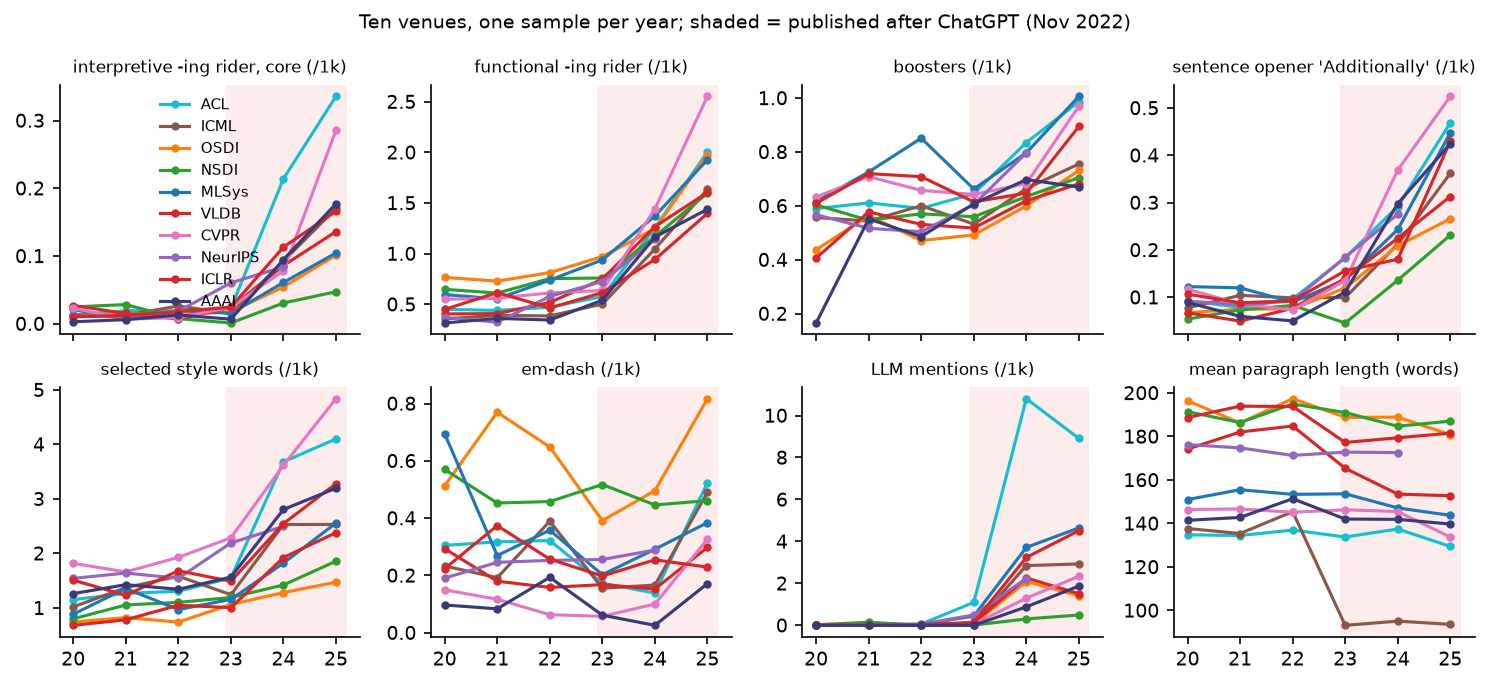
\includegraphics[width=\textwidth]{figs/fig2_series.png}
\caption{Yearly means for eight features in all ten venues. Most stay flat through 2022 and rise from 2023--24 on; em-dashes rise only in 2025, and paragraph length is flat except for ICML, whose 2023 template change splits paragraphs differently.}
\label{fig:series}
\end{figure*}

\subsection{What changed}

Table~\ref{tab:main} summarizes the measures that changed and two that did not. Four patterns stand out.

\paragraph{From reporting to interpreting.} Many sampled later papers use wording that can frame a result within the same sentence. Functional-rider proxy hits (``\ldots, enabling rapid adaptation'') went from 0.50 to 2.01 per 1,000 words and core interpretive-rider proxy hits (``\ldots, highlighting its robustness'') from 0.015 to 0.165. Both rose in all ten venues, both are almost as strong in non-LLM papers, and neither moved between 2016 and 2020. Sentences of the form ``This shows / highlights\ldots'' also rose, but less (1.9$\times$), which suggests that much of the new style is old academic style used more often.

\paragraph{From plain to elevated words.} Everyday phrasings (\textit{deal with}, \textit{look at}, \textit{keep track of}, \textit{is useful}) appear in about a third as many papers as in 2020, and their formal counterparts took their place (Table~\ref{tab:synonyms}). Among uses of \textit{important} and its elevated alternatives, \textit{crucial/critical/pivotal} went from 41\% to 73\%; \textit{facilitate} went from 21\% to 45\% of the help/facilitate pair. Non-LLM papers show nearly the same shares, and the 2016 values are close to the 2020 ones. Words became longer: the share with three or more syllables rose from 21.3\% to 25.5\%, nominalizations by about 16\%, and Flesch reading ease fell from 36.6 to 26.5 in the original v3 descriptive table (Table~\ref{tab:second}).

\paragraph{Louder and less personal.} Boosters rose and hedges fell, so boosters per hedge went from 0.27 to 0.56; \textit{we} fell by about 15\%, and so did the passive voice. In older prose, fewer \textit{we} usually meant more passives. Here, however, both declined, and the subject of the sentence is increasingly the method or the result (``This design ensures\ldots''). Claims of being first did not grow; they fell slightly (Appendix~\ref{app:equiv}).

\paragraph{Signposted blocks and packaged contributions.} Sentences opening with \textit{Additionally} became 2.9 times and with \textit{Notably} 8 times more frequent, whereas older connectives such as \textit{Moreover} and \textit{Thus} stayed flat. Authors increasingly \textit{introduce} rather than propose a system, follow its name with a one-line pitch, and describe ``extensive experiments'' (20\% $\to$ 44\% of papers).

\begin{table}[t]
\centering\footnotesize
\resizebox{\columnwidth}{!}{\begin{tabular}{l rrrr}
\toprule
Plain $\to$ elevated & 2016 & 2019--20 & 2024--26 & non-LLM \\
\midrule
match/fit $\to$ align with & 10 & 12 & 44 & 40 \\
important $\to$ crucial etc. & 39 & 41 & 73 & 70 \\
help $\to$ facilitate & 19 & 21 & 45 & 46 \\
many/various $\to$ diverse & 7 & 11 & 32 & 27 \\
improve $\to$ enhance & 14 & 16 & 37 & 36 \\
fail to $\to$ struggle to & 3 & 5 & 25 & 22 \\
ignore/miss $\to$ overlook & 1 & 2 & 20 & 18 \\
large $\to$ substantial & 21 & 22 & 38 & 38 \\
show $\to$ demonstrate & 15 & 17 & 31 & 28 \\
use $\to$ leverage/utilize & 6 & 10 & 21 & 19 \\
\bottomrule
\end{tabular}
}
\caption{Share (\%) of plain-or-elevated occurrences that use the elevated variant, averaged over venues; ``non-LLM'': 2024--26 papers that are not LLM-centred.}
\label{tab:synonyms}
\end{table}

\begin{table*}[t]
\centering\small
\begin{tabular}{l rr rrr r l}
\toprule
Measure & 2019--20 & 2024--26 & AUC & non-LLM & 16$\to$20 & Jump & Break \\
\midrule
Words with 3+ syllables & 21\% & 26\% & 0.82 & 0.79 & 0.59 & +0.77 & 2024 (47) \\
Flesch reading ease & 36.6 & 26.5 & 0.19 & 0.23 & 0.42 & -0.63 & 2024 (30) \\
Nominalizations /1k & 52.7 & 61.1 & 0.67 & 0.66 & 0.51 & +0.39 & 2024 (28) \\
Passive sentences /100 & 21.3 & 17.3 & 0.32 & 0.36 & 0.43 & -0.21 & none \\
\textit{introduce} share of contribution verbs & 16\% & 27\% & 0.65 & 0.64 & 0.53 & +0.32 & 2024 (32) \\
\textit{extensive experiments} (papers) & 20\% & 44\% & 0.62 & 0.59 & 0.54 & +0.24 & 2024 (8) \\
arXiv share of references & 23\% & 36\% & 0.63 & 0.52 & 0.66 & +0.31 & 2024 (9) \\
\bottomrule
\end{tabular}

\caption{Readability, voice, packaging and citations from the original v3 result files, pooled over ten venues (columns as in Table~\ref{tab:main}; Jump is the legacy feature-level trend coefficient in SD units). The last row is a trend that is partly topic: arXiv citations were already rising before 2020.}
\label{tab:second}
\end{table*}

\subsection{When it happened}

The yearly samples locate the change (Figure~\ref{fig:series}). On the corrected cohort's 90 venue-year means, a step at 2024 beats a linear trend by $\Delta$BIC = 95.5 for the composite-pre-SD index, and all 500 whole-venue resamples select 2024 on either candidate grid. This is selection stability under a model, not evidence that an event caused the break. The legacy per-feature fits put nine of ten venues at 2024 individually (OSDI only weakly), and NeurIPS at 2023 (Appendix~\ref{app:breaks}); venue-level timing is descriptive because publication dates need not match writing dates or PDF version dates. Some markers keep growing into 2025 (interpretive-rider proxy hits, boosters, \textit{we}), and the em-dash rises only in 2025, which may reflect later models or typesetting.

The share of papers whose style index exceeds their venue's 2019--20 95th percentile is 4\% in 2016, 6\% in 2020, 9\% in 2021 and 2022, 12\% in 2023, 42\% in 2024 and 61\% in 2025 (Figure~\ref{fig:stats}c; original v3 descriptive mapping). The 5\% threshold defines the earlier reference distribution, not an expected rate for later years. In ACL 2025 the share is 77\%; NeurIPS 2024 is 37\%.

\begin{figure*}[t]
\centering
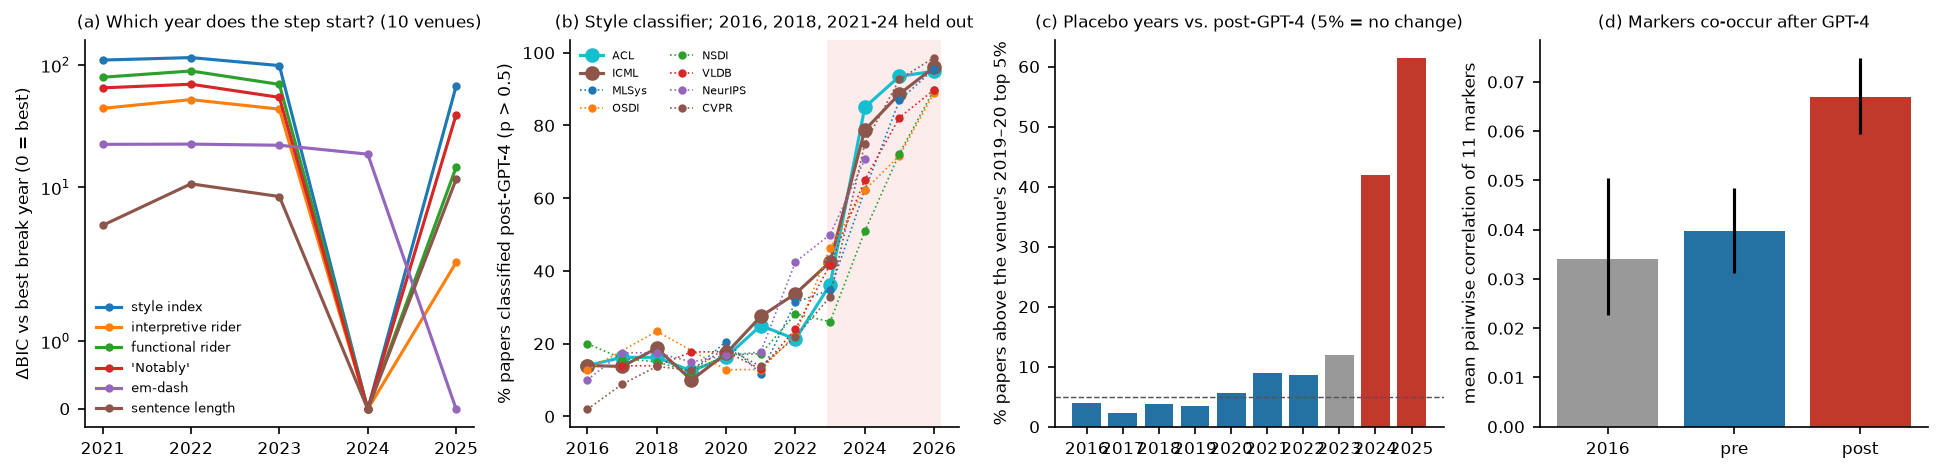
\includegraphics[width=\textwidth]{figs/fig7_statistics.png}
\caption{(a) BIC of step-plus-trend models by candidate year, relative to the best year, on venue-year means. (b) Share of papers a style-only classifier labels post-GPT-4; 2016, 2018 and 2021--24 were never seen in training. (c) Share of papers above the venue's 2019--20 95th percentile on the style index, averaged over venues. (d) Mean pairwise rank correlation among 11 markers within each era, with bootstrap 95\% intervals.}
\label{fig:stats}
\end{figure*}

\subsection{Checks against measured topic and earlier trends}

Three checks test whether the change is confined to LLM topics or continues an older trend (Table~\ref{tab:robust}); none identifies its cause. First, the AUCs computed on papers without LLM mentions are within 0.01--0.04 of the full ones for the main style features, and among the 1,127 post-GPT-4 papers that never mention LLMs the legacy style index is 2.30 SD above the 2020 mean. Papers that discuss LLMs more also have more of the new style (0.46 SD per log-unit of mentions), an association that may reflect topic and other shared influences. Second, controlling for word count, page count, references, mentions and venue leaves a legacy contrast of 2.26 SD; these measured covariates do not exhaust confounding. Third, the legacy placebo comparison of 2016 with 2020 gives a style-index AUC of 0.54 against 0.87 for 2020 with 2024--26. The 33-feature legacy classifier separates 2016 from 2020 with AUC 0.63 and 2020 from 2024--26 with 0.94; with shuffled labels it never exceeds 0.54.

The corrected 33-feature classifier reaches mean AUC 0.934 in five stratified folds when each training fold estimates its own pre-period venue baselines. In leave-one-venue-out testing it reaches mean AUC 0.922 using a pooled baseline learned from other venues, without observing target-venue papers. These splits measure era separation, not authorship detection, and neither ensures author- or source-disjointness. The legacy normalization gave a similar 0.94 within venues but used all pre-period observations to estimate baselines before splitting. In a later-specified external check, the original frozen features and model were applied without target-venue normalization or tuning to 160 preselected EMNLP 2019/20/24/25 papers, whose IDs do not overlap the original sample. Two failed the fixed body-length gate, leaving 79 papers per era. External era AUC is 0.891 (conditional paper-bootstrap 95\% interval [0.836, 0.934]); functional and interpretive clauses and \textit{Additionally/Notably} openers all have positive post-minus-pre gaps. This tests one sampled venue, not AI use or causal attribution; paper resampling does not cover shared year or composition effects. Era explains 21\% of the variance in functional clauses against 5\% for venue, while first-person use and sentence length remain mostly matters of field.

Separately, we froze a hash-selected sample of 1,200 previously unselected CVPR, ICML and NeurIPS papers (200 per venue-year in 2020 and 2025) before retrieval. All PDFs were obtained; 1,192 passed the fixed length gate. Equal-venue 2025-minus-2020 differences per 1,000 words were $+1.480$ [1.369, 1.589] for functional \textit{-ing} matches, $+0.178$ [0.156, 0.202] for core interpretive matches and $+0.439$ [0.397, 0.482] for \textit{Additionally/Notably} openers. All three prespecified interval lower bounds exceed zero. This same-field replication supports the operational pattern differences in new papers; it does not test the nine-feature index, semantic clause labels or causation (Appendix).

\begin{table}[t]
\centering\footnotesize
\resizebox{\columnwidth}{!}{\begin{tabular}{l l}
\toprule
Check & Result \\
\midrule
Placebo, 2016 vs.\ 2020: style-index AUC & 0.54 (real: 0.87) \\
Legacy placebo classifier AUC & 0.63 (real: 0.94) \\
Style index, controls for length, format, topic, venue & +2.26 SD (0.07) \\
Style index, papers with zero LLM mentions ($n$=1127) & +2.30 SD (0.08) \\
Quantile shift, 10th / 50th / 90th percentile & +0.26 / +0.59 / +0.97 SD \\
Pooled AUC with zero-LLM-mention post papers & 0.84 (all papers: 0.87) \\
Legacy classifier CV / LOVO AUC & 0.94 / 0.92 \\
Classifier with shuffled labels: mean / max AUC & 0.51 / 0.54 \\
Pooled AUC, dropping any one venue & 0.87--0.88 \\
Marker correlation, 2019--20 vs.\ 2024--26 (mean $\rho$) & 0.040 vs.\ 0.067 \\
\bottomrule
\end{tabular}
}
\caption{Original v3 robustness and placebo checks. Classifier rows used legacy full-data normalization; corrected fold-local and unseen-venue AUCs are reported in the text. SD: the venue's pre-LLM standard deviation.}
\label{tab:robust}
\end{table}

\subsection{How widespread}

The whole distribution moved, but unevenly. A quantile regression of the style index on era (with venue effects) gives shifts of $+0.26$ SD at the 10th percentile, $+0.59$ at the median and $+0.97$ at the 90th. The regenerated v3 score table puts the post-era 10th percentile above the pre-era median in six of ten venues. The omitted VLDB-2016 controls do not enter either the 2019--20 pre baseline or the 2024--26 post cohort used for this comparison. Within each era, papers also became more alike in their function-word profiles, by 3--17\% in all ten venues, while their vocabulary grew richer (MATTR 0.45 $\to$ 0.49). Before LLMs the markers varied almost independently of each other; in later publication cohorts they became modestly correlated (mean $\rho$ 0.040 $\to$ 0.067, Figure~\ref{fig:stats}d). Correlation alone cannot identify a shared cause.

Finally, excess vocabulary~\citep{kobak2024delving} describes how selected markers spread; it is not a lower bound on LLM assistance. We chose marker words on a random half of the papers (by hash of paper id) and measured on the other half the share using three or more. This measure rises across the sampled venues, but other changes in topic, editing or author composition could produce the same pattern.

\subsection{What did not change}

Sentence length (21.9 vs.\ 21.7 words), semicolons, questions, the length of introductions and related-work sections, and the number of figures are all within $\pm$0.2 SD of 2020 by an equivalence test (Appendix~\ref{app:equiv}). Variability of sentence length fell slightly ($-0.22$ SD after trend adjustment), far less than the register changes, so ``uniform sentence length'' is not a useful sign of LLM writing in CS. Triads and the em-dash show no jump beyond their trends. The largest structural changes trace to venue policy or to older trends: Limitations sections went from 1\% to 66\% of ACL papers in 2023, the year they became mandatory; PDFs grew because proceedings began to include appendices; and references and arXiv citations were already rising between 2016 and 2020.

\subsection{Can today's LLMs reproduce the shift?}

One mechanism probe edits pre-period text with current LLMs and checks whether the same features move. We sampled 160 held-out paragraphs from 2019--20 papers (20 per venue, 80--200 words, no equations or LLM mentions) and 160 paragraphs from 2024--26 papers as the target. The Claude Haiku and Sonnet models available through the Claude Code CLI in October 2026 edited every paragraph under five requests (fix grammar only; polish; improve for a top conference; rewrite to sound more polished and professional; and write a fresh paragraph from bullet notes extracted from the original), and Opus applied ``polish'' to 80 paragraphs.

\begin{table*}[t]
\centering\small
\begin{tabular}{l r rrrrrrr}
\toprule
Measure & Corpus & S:grammar & S:polish & S:improve & S:rewrite & S:draft & H:rewrite & O:polish \\
\midrule
Functional riders & +1.21 & 0.00 & -0.13 & -0.98 & -0.28 & -1.73 & -0.10 & -2.79 \\
\textit{Additionally/Notably} & +1.66 & 0.00 & +0.02 & -1.08 & -0.37 & -1.08 & -1.08 & 0.00 \\
Style words & +0.44 & 0.00 & -0.03 & -0.07 & -0.20 & -0.15 & -0.15 & -0.23 \\
Elevated synonyms & +0.32 & 0.00 & -0.05 & -0.08 & +0.06 & -0.21 & +0.07 & -0.22 \\
Boosters & +0.17 & 0.00 & +0.13 & +0.21 & +0.30 & +0.02 & +0.46 & +0.24 \\
Hedges & -0.17 & 0.00 & -0.02 & -0.15 & -0.15 & -0.07 & -0.15 & +0.03 \\
Passive voice & -0.32 & 0.00 & -0.15 & -0.34 & -0.17 & -0.51 & -0.19 & -0.32 \\
Flesch (diff./10) & -0.92 & -0.02 & +0.01 & +0.02 & -0.28 & +0.62 & -0.28 & +0.24 \\
\midrule
Spearman with corpus & -- & +0.32 & +0.12 & -0.15 & +0.02 & -0.07 & +0.12 & -0.32 \\
\bottomrule
\end{tabular}

\caption{Rewrite calibration: log ratio of each measure in the edited text against the original 2019--20 paragraphs (Flesch: difference divided by 10). ``Corpus'' is the real change between 2019--20 and 2024--26 paragraphs. S/H/O: Claude Sonnet, Haiku, Opus.}
\label{tab:calib}
\end{table*}

The current models do not reproduce the full signature (Table~\ref{tab:calib}, Figure~\ref{fig:calib}). They raise boosters and lower hedges and passive voice, as the corpus did, and the heavy ``rewrite'' request lowers readability and slightly raises elevated synonyms. However, every editing request reduced functional clauses and \textit{Additionally/Notably} openers instead of increasing them, no rewrite added a single interpretive clause, and the rank correlation between rewrite effects and corpus effects ranged from $-0.32$ to $+0.32$. The grammar-only control changed nothing.

Historical edits provide a separate mechanism check. In the April 2023--April 2024 WildChat snapshot~\citep{zhao2024wildchat}, 837,989 conversations yield 478,498 English conversations and 677 eligible 80--200-word editing pairs; 64 pairs (56 GPT-3.5, eight GPT-4) meet the final academic filter. Selection was revised three times before feature computation; two revisions widened selection after academic counts of 16 and 28 were seen. In this \emph{primary academic subset}, edit/original log ratios are $+0.06$ [--0.42, 0.74] for functional clauses, $+1.69$ [0.00, 2.53] for interpretive clauses, and $+1.41$ [0.64, 2.77] for \textit{Additionally/Notably} openers (paired-bootstrap 95\% intervals). The frozen three-feature readout is \textbf{inconclusive}; the functional interval crosses zero and the interpretive interval touches it. The exploratory all-English set gives $+0.44$ [0.23, 0.65], $+0.67$ [0.17, 1.21] and $+1.20$ [0.88, 1.52], respectively, and a rank correlation of $+0.65$ with the corpus's 15-feature changes. It also increases the famous ChatGPT words and first-person pronouns, which move oppositely in the CS corpus. The WildChat and Claude calibrations differ in people, passages, requests and selection, so their contrast cannot isolate model generation. These observations show that selected historical editing responses \emph{could} produce many measured changes, not that studied paper authors used the tools. The protocol, selection deviations and exclusion counts are archived with the aggregate results.

\begin{figure*}[t]
\centering
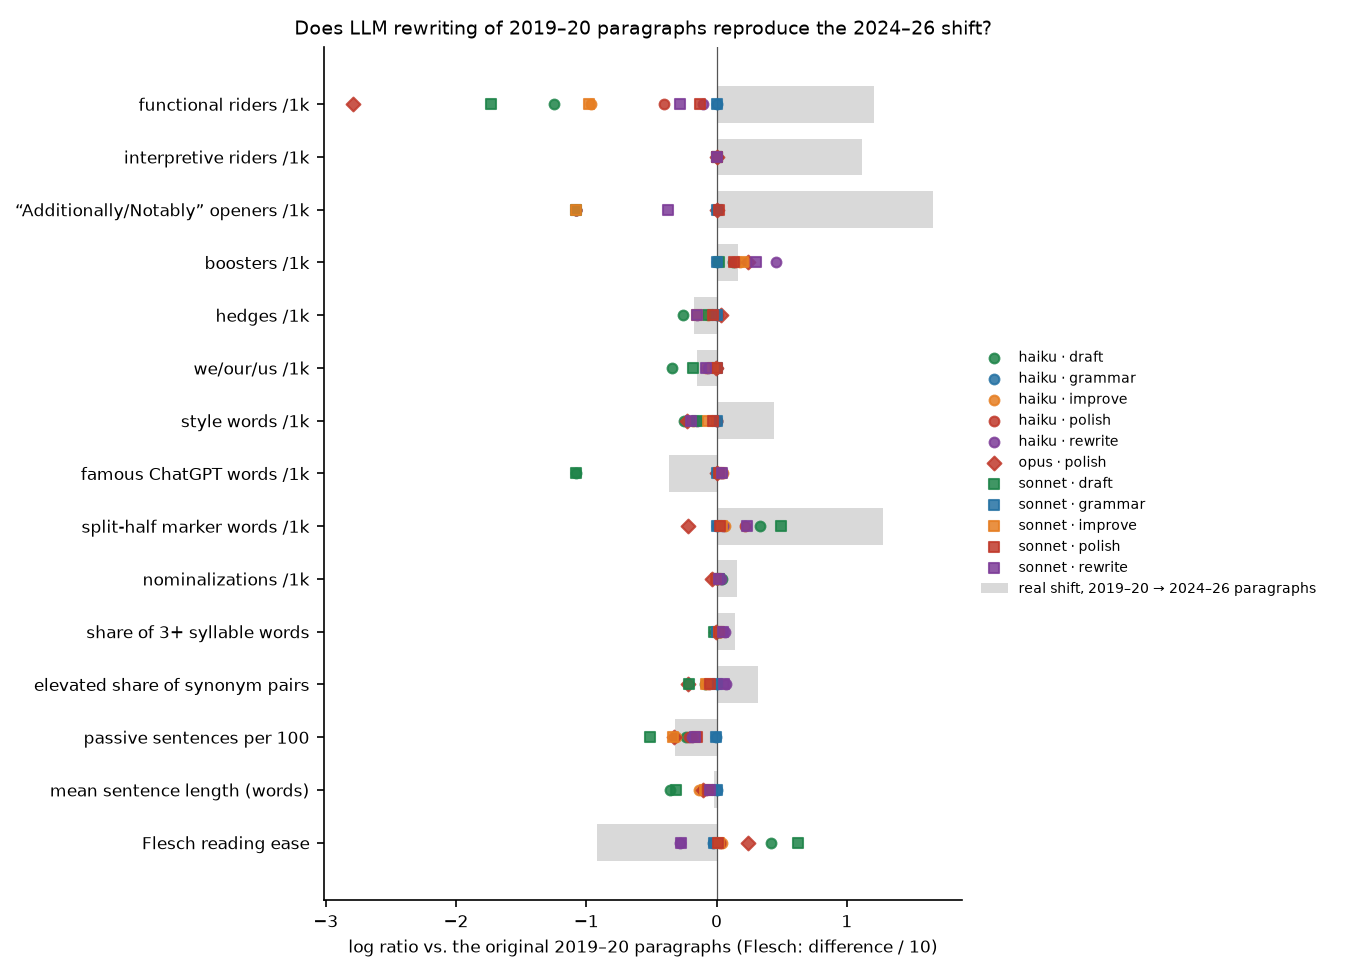
\includegraphics[width=0.82\textwidth]{figs/fig8_rewrite_calibration.png}
\caption{Real change from 2019--20 to 2024--26 paragraphs (grey bars) and the change produced by Claude models editing the same 2019--20 paragraphs (markers).}
\label{fig:calib}
\end{figure*}

\section{Discussion}

The shift we measure is in register and stance, concentrated in the sentences that frame and summarize a contribution: interpretive-rider proxy hits are densest in conclusions, abstracts and related work, and \textit{Additionally/Notably} in Limitations sections. Several measured sentence and section-length outcomes show small differences; we did not detect a comparable jump in novelty claims, whereas section counts changed with venue policies. For authors, the sampled 2025 cohort has a distinguishable aggregate register, and the plain verbs of 2020 papers remain perfectly acceptable at the same venues. For reviewers, the base rate matters: with 40--80\% of 2025 papers above the 2020 range, a single ``LLM-sounding'' word says almost nothing about a paper, and style should never be used to rank or accuse individual papers. For detectors, the features that separate the sampled eras in CS include participial-rider proxies, connectives, synonym choice and stance, while the biomedical tell-tale words and sentence-length uniformity are weak.

\section{Limitations}

Our design is observational: the change coincides with LLM availability, persists under measured trend, topic-flag and placebo checks, and spans fields, but we never observe anyone using an LLM, and current-model rewrites did not reproduce the clause and opener changes. The rider regex has not been validated against human clause labels and may count lists or embedded modifiers; its rates should not be read as verified sentence-final clause rates. A two-agent blind pilot is descriptive, not human gold, and was too sparse to validate the rare core interpretive category (Appendix). Features and lexicons were refined after inspecting this corpus; fold-local preprocessing removes one leakage path but does not remove optimism from global feature selection. The same-field expansion confirms three fixed pattern-count differences in disjoint sampled papers, not the selected nine-feature index or an independent author population. The later EMNLP sample tests fixed measurements in one new venue; a separately frozen PLOS Genetics check did not meet its three-feature joint criterion (Appendix). These checks do not confirm broad cross-field generalization or the nine-feature index effect. Imitation, grammar tools, changing authors and shared calendar-year shocks could all contribute. An exploratory ACL control exactly matches 760 papers to official metadata but links only 11 people and 31 papers across eras; its author-fixed-effect style-lexicon difference is +0.912 per 1,000 words, versus +2.704 in the original ACL cohort. Uneven identity coverage and this small selected panel do not establish author-composition robustness. Text extraction from PDFs is imperfect; ICML's 2023 template changes paragraph splitting. Seven papers were omitted through download or link errors and all seven were recovered in a separate post-result sensitivity check. The same three feature definitions as the PLOS check, applied here to the original CS corpus, produced small shifts, but the trend-adjusted index and changepoint were not recomputed; the 1,500-word gate removes 14/80 AAAI 2016 and 12/80 AAAI 2018 papers, versus none in AAAI 2020--26. A version-pinned ICLR source/PDF sensitivity retained 20 of 24 selected pairs (11 pre, 9 post): all nine measured era-gap directions agreed, but the em-dash gap was +0.367 versus +0.617 per 1,000 words and source parsing retained only about 86\% as many words. This small heuristic comparison does not prove extraction equivalence. Of 418 pre-2023 ICLR PDFs, 18 have explicit later arXiv version stamps; excluding them or all ICLR preserves the direction of the corrected index contrast but cannot rule out other revisions. Our LLM-topic flag is a word count. COLM and EuroSys rely on arXiv versions and have no pre-era baselines.

\section*{Ethics Statement}

We analyze published papers at the level of venues and years. We do not identify, score or rank individual papers or authors. Repository artifacts use hashed paper identifiers and do not include PDFs or extracted text; public release remains subject to review. Examples of the patterns in this paper and on its companion website are written by us, except for a guessing game on the website that shows short excerpts from ACL Anthology papers under their CC BY 4.0 license, each credited after the guess with a note that the label is only the publication date. The contemporary rewrite calibration sent held-out published-paper paragraphs through the Claude Code CLI; the historical calibration uses an existing public conversation dataset and commits only aggregate measurements.

\bibliographystyle{plainnat}
\bibliography{refs}

\appendix
\onecolumn

\section{Per-venue break years}
\label{app:breaks}
\begin{table}[h]
\centering\small
\begin{tabular}{l llll}
\toprule
Venue & Style index & Functional riders & Interpretive riders & \textit{Notably,} \\
\midrule
ACL & 2024 (29) & 2024 (12) & 2024 (18) & 2024 (27) \\
CVPR & 2024 (12) & 2025 (14) & 2025 (26) & 2024 (14) \\
ICML & 2024 (17) & 2024 (12) & 2024 (11) & 2024 (12) \\
NeurIPS & 2023 (8) & 2024 (7) & 2023 (15) & 2024 (4) \\
VLDB & 2024 (14) & 2024 (14) & 2024 (11) & 2024 (28) \\
MLSys & 2024 (12) & 2025 (4) & 2025 (5) & 2024 (14) \\
OSDI & 2024 (3) & 2025 (13) & 2025 (9) & 2023 (9) \\
NSDI & 2024 (16) & 2024 (11) & 2024 (5) & 2024 (18) \\
ICLR & 2024 (16) & 2025 (8) & 2024 (15) & 2024 (19) \\
AAAI & 2024 (18) & 2024 (18) & 2024 (10) & 2024 (18) \\
\bottomrule
\end{tabular}

\caption{Best step year for each venue fit separately, with $\Delta$BIC against a linear trend in parentheses. Single-venue fits use 7--10 yearly means, so $\Delta$BIC is smaller than in the pooled fit.}
\end{table}

\section{Equivalence tests}
\label{app:equiv}
\begin{table}[h]
\centering\small
\begin{tabular}{l r c c}
\toprule
Measure & Shift (SD) & 90\% CI & Within $\pm$0.2 SD \\
\midrule
Sentence length & -0.05 & [-0.10, 0.00] & yes \\
Sentence-length CV & -0.11 & [-0.16, -0.05] & yes \\
\textit{not only\ldots but also} & +0.17 & [+0.11, +0.24] & no \\
Lists of three & +0.40 & [+0.33, +0.46] & no \\
Semicolons & +0.13 & [+0.08, +0.19] & yes \\
Questions & -0.05 & [-0.10, +0.01] & yes \\
\textit{first} / \textit{to our knowledge} & -0.14 & [-0.19, -0.08] & yes \\
Number of sections & +0.28 & [+0.22, +0.34] & no \\
Introduction length & -0.13 & [-0.19, -0.08] & yes \\
Related-work length & -0.07 & [-0.13, -0.02] & yes \\
Number of figures & +0.12 & [+0.07, +0.18] & yes \\
\bottomrule
\end{tabular}

\caption{Shift from 2019--20 to 2024--26 in pre-LLM SD units, pooled over venues by inverse variance, with 90\% confidence intervals; ``yes'' means the two one-sided tests reject a change larger than 0.2 SD.}
\end{table}

\section{Effect sizes for all measures}
\begin{figure}[H]
\centering
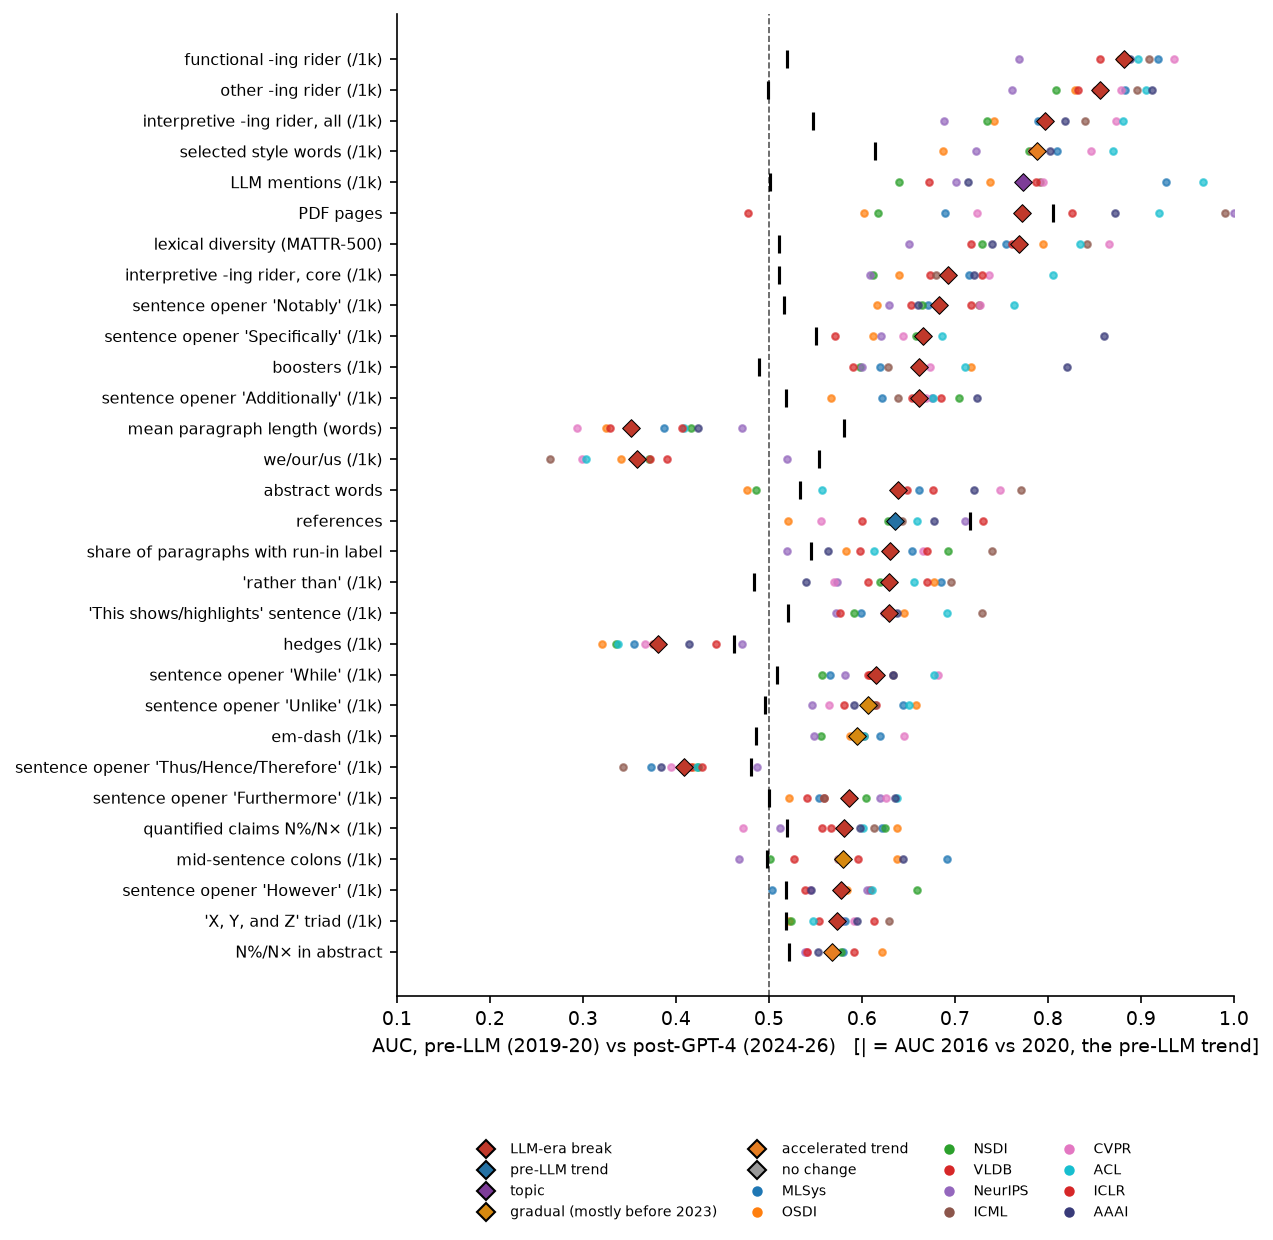
\includegraphics[width=0.78\textwidth]{figs/fig1_effects.png}
\caption{The 30 largest changes. Diamonds: mean AUC over ten venues, coloured by attribution; dots: individual venues; black tick: AUC between 2016 and 2020.}
\end{figure}

\clearpage
\section{Additional field and measurement checks}
In a separately frozen same-field expansion, hash ranking selected 200 source IDs in each 2020/2025 cell of CVPR, ICML and NeurIPS after excluding the original list. All 1,200 PDFs were retrieved, their hashes committed before extraction, and eight failed the unchanged 1,500-body-word gate without replacement. Among 1,192 eligible papers, the three fixed 2025-minus-2020 pattern differences per 1,000 words, equal-weighted across venues, were functional \textit{-ing} $+1.480$ [1.369, 1.589], core interpretive \textit{-ing} $+0.178$ [0.156, 0.202] and \textit{Additionally/Notably} openers $+0.439$ [0.397, 0.482] (2,000 within-cell paper-bootstrap draws; 95\% intervals). All three lower bounds exceeded zero, meeting the frozen joint rule; each venue-level interval was also positive. An independent check confirmed all PDF hashes, recomputed feature values from the cached extracted text and reproduced the intervals with separate statistical code. This check uses new papers at three already studied CS venues and fixed operational counts; source IDs are disjoint, but authors and topics may overlap. It does not validate semantic clause labels, the nine-feature index, other fields or an AI cause.

In a separately frozen PLOS Genetics check, all 80 selected articles (20 each in 2019, 2020, 2024 and 2025) passed retrieval, extraction and the fixed body-length gate. The three preselected post-minus-pre gaps per 1,000 words were functional \textit{-ing} $+0.194$ [0.032, 0.348], core interpretive \textit{-ing} $+0.040$ [--0.003, 0.081], and \textit{Additionally/Notably} openers $+0.124$ [--0.049, 0.281] (conditional 95\% paper-bootstrap intervals). The joint criterion required all three intervals to exclude zero positively; it failed. This is mixed, inconclusive transfer evidence in one new field, not an AI-use test or evidence of no change.

A blind pilot gave two independent sessions of the same agent family 320 uniformly sampled and 91 detector-enriched sentences, without era, venue or detector labels. Of five functional-vocabulary detector heads in the random sample, three matched both reviewers' confident semantic and attachment judgments and two lacked a confident joint head; the enriched sample gave 26 matches and ten unmatched among 36 heads. Only one core-interpretive head appeared in the enriched sample and none in the random sample. Reviewer uncertainty affected 32 and 33 of 320 random sentences, respectively. Shared agent errors and uncertainty preclude an accuracy, precision or recall estimate; disputed items await human adjudication.

\section{Reproducibility}
The repository contains analysis scripts, the sampled-paper list, aggregate outputs and an anonymous numerical feature snapshot with source and code hashes. An isolated rerun regenerated all 36 corrected statistical CSVs byte-for-byte from the public numeric snapshot. A same-machine full rerun re-extracted all 9,472 analyzed cached PDFs: text records and features exactly match the private cache and public numeric snapshot; 23 sampled source re-downloads were byte-identical. This verifies determinism given the same PDF bytes and Poppler 26.04.0, not source stability or feature validity. All seven papers lost to download or link errors were recovered separately and passed the fixed length gate; six enter post-period cells and OSDI 2023 only the yearly series. Adding them changes the ten-venue equal-weight simple post-minus-pre gaps by at most $+0.0015$ per 1,000 words across the same three feature definitions as the PLOS check, applied here to the original CS corpus; in the two affected pre/post venues (AAAI and NSDI), each recovered-cohort point estimate stayed within its original-cohort bootstrap interval; no interval was computed for the ten-venue mean. The trend-adjusted index and changepoint were not recomputed. The original main-cohort estimates were not altered. The published PDF-hash manifest has 9,626 rows, including hashes for 9,622 cached PDFs (26,498,546,116 bytes) and four without a PDF, and allows later source checks; unversioned arXiv and GitHub-main URLs can change. An outside rerun needs the frozen paper list, version-matched PDFs, Poppler and the hash-matched extraction helper; the legacy driver still writes into the result directory. The current rewrite calibration invokes the Claude Code CLI. Historical WildChat pair selection and aggregate analysis are reproducible from the pinned public dataset revision and released scripts; pair text is not committed.

\end{document}
